\documentclass[11pt,a4paper]{article}

% -----------------------------------------------------------------------
% Packages
% -----------------------------------------------------------------------
\usepackage[T1]{fontenc}
\usepackage[utf8]{inputenc}
\usepackage[margin=2.5cm]{geometry}
\usepackage{amsmath,amssymb,amsthm}
\usepackage{graphicx}
\usepackage{subcaption}
\usepackage{booktabs}
\usepackage{hyperref}
\usepackage{cleveref}
\usepackage{microtype}
\usepackage{parskip}
\usepackage[ruled,vlined]{algorithm2e}
\usepackage{xcolor}

% -----------------------------------------------------------------------
% Theorem environments
% -----------------------------------------------------------------------
\newtheorem{theorem}{Theorem}
\newtheorem{lemma}{Lemma}
\newtheorem{definition}{Definition}

% -----------------------------------------------------------------------
% Macros
% -----------------------------------------------------------------------
\newcommand{\OPT}{\phi_{\mathrm{OPT}}}
\newcommand{\Dx}{D(x)}
\newcommand{\phiC}{\phi(C)}
\newcommand{\E}{\mathbb{E}}

% -----------------------------------------------------------------------
% Title
% -----------------------------------------------------------------------
\title{%
  \textbf{k-means++: The Advantages of Careful Seeding}\\[4pt]
  \large Assignment 5: Clustering and Initialization\\
  Statistical Methods for Machine Learning, A.Y. 2025/26
}
\author{Mohamed Yousif}
\date{June 2026}

% -----------------------------------------------------------------------
\begin{document}
% -----------------------------------------------------------------------
\maketitle

\begin{abstract}
We implement and empirically evaluate Lloyd's k-means algorithm under two
initialization strategies: uniform random seeding and the k-means++ D\textsuperscript{2}-weighted
seeding of Arthur and Vassilvitskii~\cite{arthur2007kmeans}.
Experiments on synthetic Gaussian blobs (2-D and 20-D), the Credit Card Segmentation
Dataset (8{,}950 customer records, 17 features), and a 5{,}000-image MNIST
subset reduced to 50 PCA dimensions show that the advantage of k-means++ is
context-dependent: it achieves inertia ratios of 3.09$\times$ ($d=2$) and
4.54$\times$ ($d=20$) over random seeding on synthetic data, and produces
better-aligned clusters on MNIST despite equal inertia, but on easy real-world
instances with small $k$ the simpler baseline is equally reliable.
All algorithms are implemented from scratch using NumPy.
\end{abstract}

% -----------------------------------------------------------------------
\section{Introduction}
% -----------------------------------------------------------------------

Clustering is an unsupervised learning task whose goal is to partition a
dataset $\mathcal{X} = \{x_1, \dots, x_n\} \subset \mathbb{R}^d$ into
$k$ groups that are compact and well-separated.
The standard approach, Lloyd's algorithm (often called k-means), minimises
the \emph{k-means objective}
\[
  \phiC = \sum_{x \in \mathcal{X}} \min_{c \in C} \|x - c\|^2,
\]
where $C = \{c_1, \dots, c_k\}$ is the set of cluster centres.
Although Lloyd's algorithm is guaranteed to converge, it finds only a local
minimum.
Theorem~1.1 of Arthur and Vassilvitskii~\cite{arthur2007kmeans} shows that
random initialisation can yield solutions that are arbitrarily worse than
the global optimum: for any $k$ and any $n$, there exist inputs on which
the expected cost is $\Omega(\log k) \cdot \OPT$.

The k-means++ paper addresses this weakness with a simple randomised
initialisation scheme, D\textsuperscript{2}-sampling (Algorithm~1 in the
paper), and proves an $O(\log k)$ approximation guarantee before any
Lloyd iteration is run (Theorem~3.1).
This report shows how carefully designed randomness can tame non-convexity
and stabilise a learning algorithm that is otherwise highly sensitive to
its starting configuration.

% -----------------------------------------------------------------------
\section{Algorithms}
% -----------------------------------------------------------------------

\subsection{Lloyd's Algorithm (k-means)}

Given initial centres $C^{(0)}$, Lloyd's algorithm alternates two steps:

\begin{enumerate}
  \item \textbf{Assign (E-step).} For each $x \in \mathcal{X}$, set
    $\ell(x) = \arg\min_{j} \|x - c_j^{(t)}\|^2$.
  \item \textbf{Update (M-step).} For each cluster $j$, set
    $c_j^{(t+1)} = \frac{1}{|S_j|}\sum_{x \in S_j} x$,
    where $S_j = \{x : \ell(x) = j\}$.
\end{enumerate}

Both steps can only decrease $\phiC$, so the algorithm converges in a finite
number of iterations~\cite{arthur2007kmeans} (Section~2).
Convergence is detected when the maximum coordinate-wise centroid shift
falls below a tolerance $\tau$ (set to $10^{-4}$ in our implementation).

\subsection{k-means++ Initialisation}

\begin{algorithm}[H]
\caption{k-means++ seeding (Algorithm~1, Arthur \& Vassilvitskii 2007)}
\KwIn{Dataset $\mathcal{X}$, number of clusters $k$}
\KwOut{Initial centres $C = \{c_1, \dots, c_k\}$}
Choose $c_1$ uniformly at random from $\mathcal{X}$\;
\For{$i = 2, \dots, k$}{
  Compute $\Dx = \min_{c \in C} \|x - c\|^2$ for all $x \in \mathcal{X}$\;
  Sample $c_i \sim \mathcal{X}$ with probability $\Pr[x] = \Dx / \sum_{x'} D(x')^2$\;
  Add $c_i$ to $C$\;
}
Proceed with standard Lloyd's algorithm from $C$\;
\end{algorithm}

The key idea is \emph{D\textsuperscript{2}-sampling}: each new centre is
chosen with probability proportional to the squared distance to the nearest
already-chosen centre.
This pushes centres apart and ensures the initial configuration covers the
data more evenly than uniform random sampling.

\begin{theorem}[Theorem~3.1, \cite{arthur2007kmeans}]
  Let $C$ be the set of centres produced by Algorithm~1.
  Then $\E[\phiC] \leq 8(\ln k + 2)\,\OPT$.
\end{theorem}

The proof proceeds by induction using two auxiliary lemmas (Lemmas 3.2
and~3.3 in the paper).
Lemma~3.2 shows that for any optimal cluster $A^*$ whose centre has not
yet been chosen, one round of D\textsuperscript{2}-sampling reduces the
expected contribution of $A^*$ to the total cost by a constant factor.
Lemma~3.3 handles the case where some centres from $A^*$ have already been
covered.

\subsection{Implementation Notes}

All algorithms are implemented from scratch in \texttt{src/}.
\begin{itemize}
  \item \texttt{src/distance.py}: squared Euclidean distance primitives using
    the $\|x - c\|^2 = \|x\|^2 - 2x \cdot c + \|c\|^2$ expansion to avoid
    explicit loops over centers.
  \item \texttt{src/init.py}: \texttt{random\_init} and \texttt{plusplus\_init}
    with a shared interface; the \texttt{KMeans} class selects between them.
  \item \texttt{src/kmeans.py}: \texttt{KMeans} class with a pluggable
    initialisation argument, \texttt{n\_init} independent restarts (keeping
    the best inertia), and a \texttt{fit\_with\_history} method for
    convergence curve plotting.
  \item External libraries: \texttt{numpy} for computation,
    \texttt{matplotlib} for plotting, \texttt{scikit-learn} only for
    \texttt{fetch\_openml} (MNIST download) and \texttt{PCA}
    (dimensionality reduction utility).
\end{itemize}

% -----------------------------------------------------------------------
\section{Datasets}
% -----------------------------------------------------------------------

\subsection{Synthetic Gaussian Blobs}

Controlled experiments use isotropic Gaussian blobs generated with
\texttt{src/data.make\_blobs}.
Two settings are tested: well-separated ($d=2$, $\sigma=0.8$, $k=5$)
and high-dimensional ($d=20$, $\sigma=0.8$, $k=5$), each with $n=2{,}000$
points.
A third setting with $\sigma=2.5$ (overlapping clusters) provides the
extension experiment.

\subsection{Credit Card Segmentation Dataset}

The Credit Card Segmentation Dataset~\cite{ccgeneral} contains $n=8{,}950$ credit-card
customer records with $p=17$ numeric features covering balances, purchase
behaviour, cash-advance patterns, repayment rates, credit limits, and tenure.
Missing values are limited: \texttt{MINIMUM\_PAYMENTS} (${\approx}3.5\%$)
and \texttt{CREDIT\_LIMIT} (1 row) are median-imputed.
All features are standardised to zero mean and unit variance before any
distance computation.

\subsection{MNIST}

A 5{,}000-image random subset of MNIST~\cite{lecun1998mnist} (originally
$n=70{,}000$, $d=784$) is used for the high-dimensional extension.
Pixel values are normalised to $[0,1]$ and then projected to 50 PCA
components, which retain approximately $85\%$ of the total variance.
The natural choice of $k=10$ aligns with the ten digit classes, allowing
a sanity-check via cluster purity.

% -----------------------------------------------------------------------
\section{Experimental Setup}
% -----------------------------------------------------------------------

The core comparison isolates the effect of initialisation by running each
algorithm with \textbf{one restart} (\texttt{n\_init=1}) over many
independent trials.
Each trial uses a distinct random seed derived from a base seed, so the
distribution of outcomes directly reflects the quality of the seeding
strategy.

\paragraph{Metrics.}
\begin{itemize}
  \item \textbf{Inertia} $\phiC$ (primary): the k-means objective.
    Lower values indicate tighter, better-separated clusters.
  \item \textbf{Number of Lloyd iterations} (secondary): lower means the
    initialisation starts closer to a good solution.
  \item \textbf{Cluster purity} (sanity check, MNIST only): fraction of
    points in each cluster dominated by one true digit label.
\end{itemize}

\paragraph{Multi-restart runs.} When producing a single \emph{best solution}
for cluster profiling (Section~\ref{sec:results-real}), we use
\texttt{n\_init=10} and keep the run with the lowest inertia, consistent
with standard practice and the recommendation implied in Section~4 of the paper.

All experiments are seeded with \texttt{random\_state=42} and are fully
reproducible by re-running the notebooks in order.

% -----------------------------------------------------------------------
\section{Results: Synthetic Data}
\label{sec:results-synth}
% -----------------------------------------------------------------------

\begin{figure}[h]
  \centering
  \begin{subfigure}[b]{0.48\textwidth}
    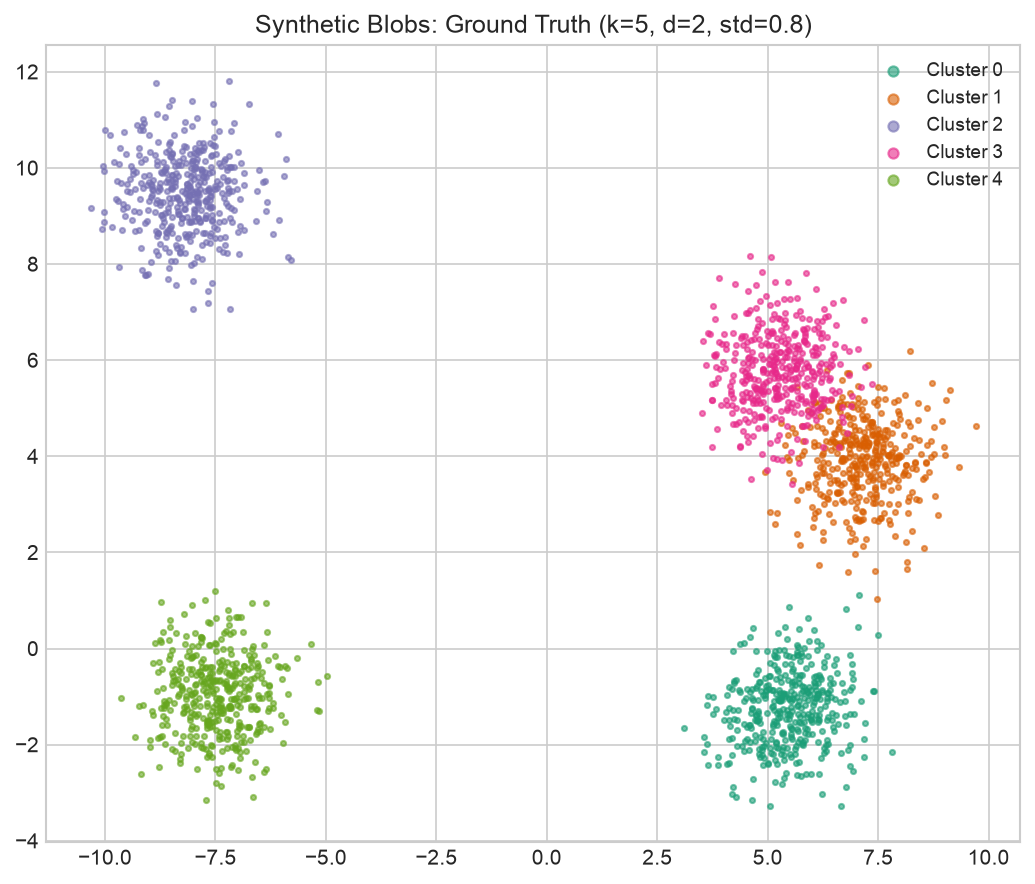
\includegraphics[width=\textwidth]{figures/synth_blobs_gt.png}
    \caption{Ground-truth clusters ($d=2$, $\sigma=0.8$, $k=5$).}
  \end{subfigure}
  \hfill
  \begin{subfigure}[b]{0.48\textwidth}
    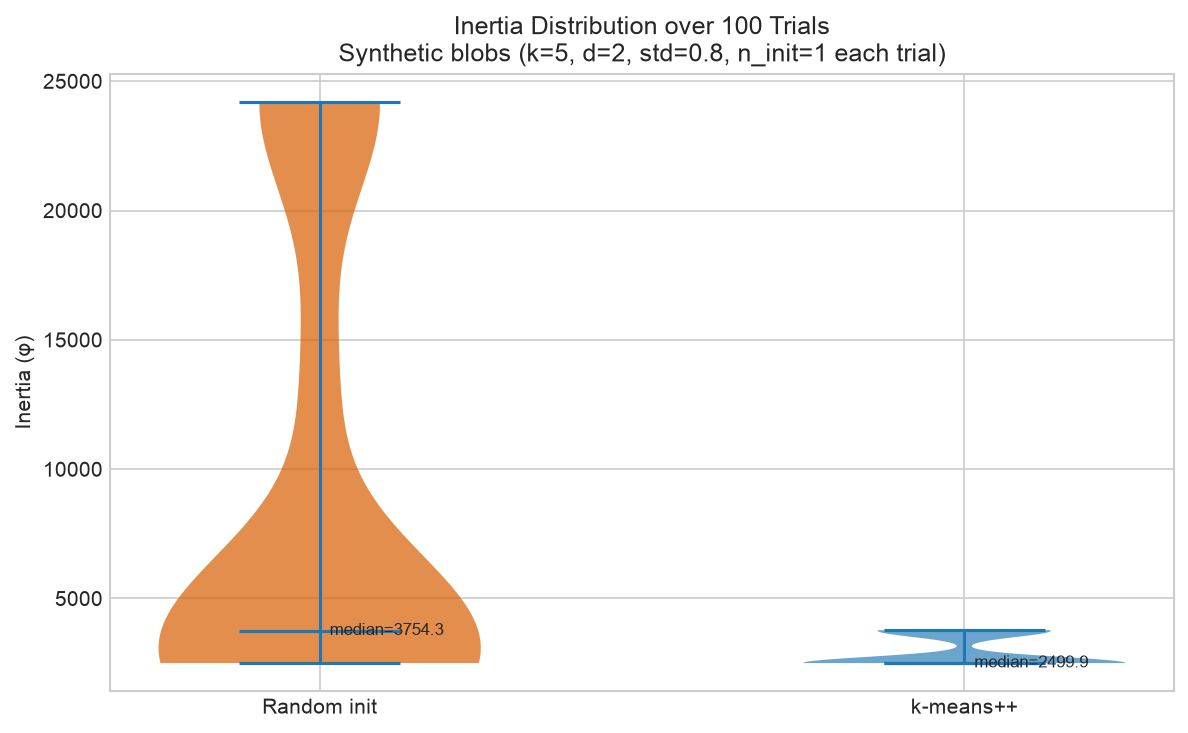
\includegraphics[width=\textwidth]{figures/synth_inertia_violin.png}
    \caption{Inertia distribution over 100 trials ($n_\text{init}=1$).}
  \end{subfigure}
  \caption{Well-separated synthetic blobs: data structure and initialisation effect.}
  \label{fig:synth-violin}
\end{figure}

\Cref{fig:synth-violin} shows the inertia distributions for 100 independent
single-restart trials on the 2-D blob dataset.
k-means++ achieves a lower median inertia and a substantially smaller spread
compared to random initialisation, consistent with the $O(\log k)$ guarantee
of Theorem~3.1.

The observed mean inertia ratio (random / k-means++) is \textbf{3.09$\times$}
for $d=2$ (random mean $\phi=9{,}089.8$, k-means++ mean $\phi=2{,}938.6$) and
\textbf{4.54$\times$} for $d=20$ ($\phi=198{,}390.6$ vs $43{,}732.2$).
The advantage grows with dimensionality, confirming that random seeding is
progressively more likely to miss cluster regions as $d$ increases;
this is shown directly in \Cref{fig:synth-hd}.

\begin{figure}[h]
  \centering
  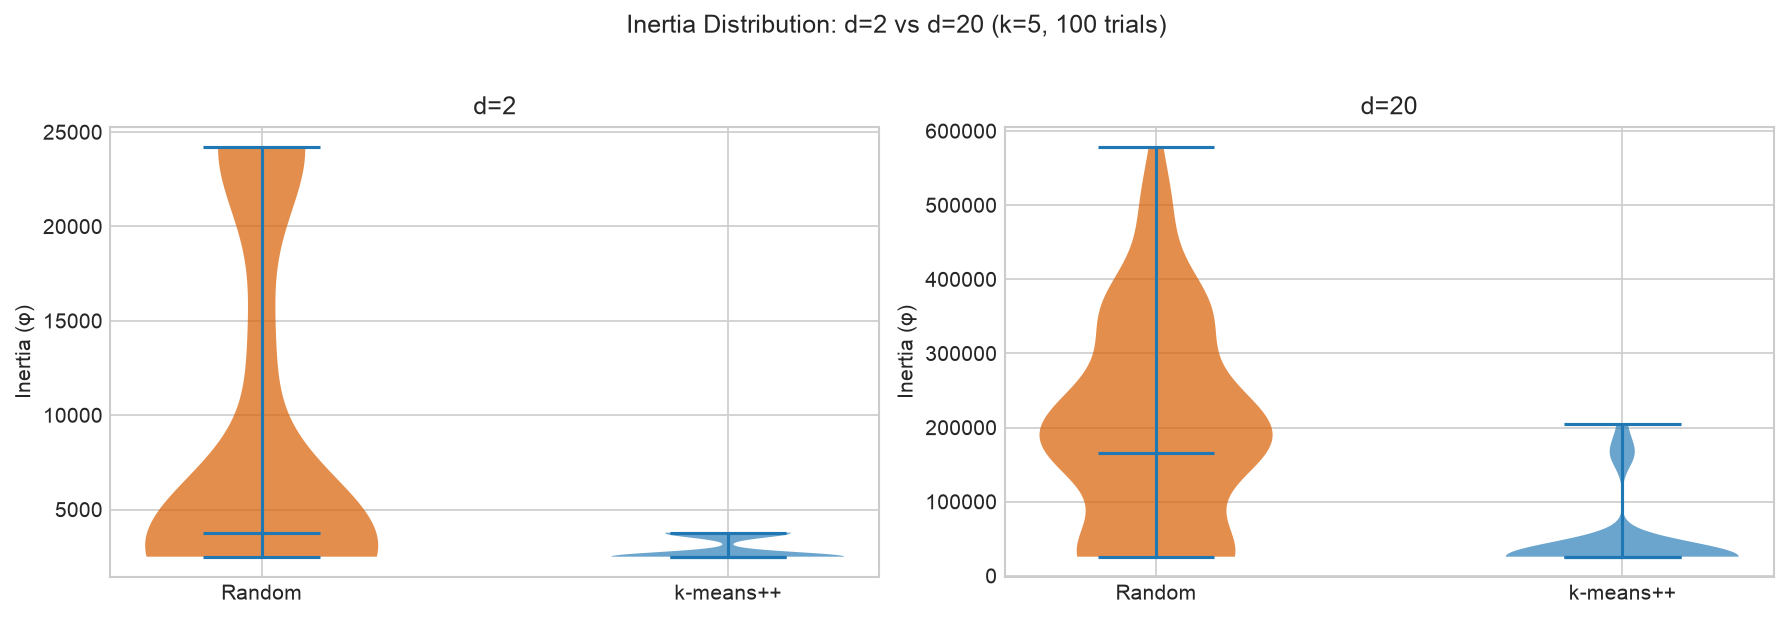
\includegraphics[width=0.85\textwidth]{figures/synth_hd_comparison.png}
  \caption{Inertia distributions for $d=2$ (left) and $d=20$ (right) over 100 trials.
           The gap widens substantially in higher dimensions.}
  \label{fig:synth-hd}
\end{figure}

\begin{figure}[h]
  \centering
  \begin{subfigure}[b]{0.48\textwidth}
    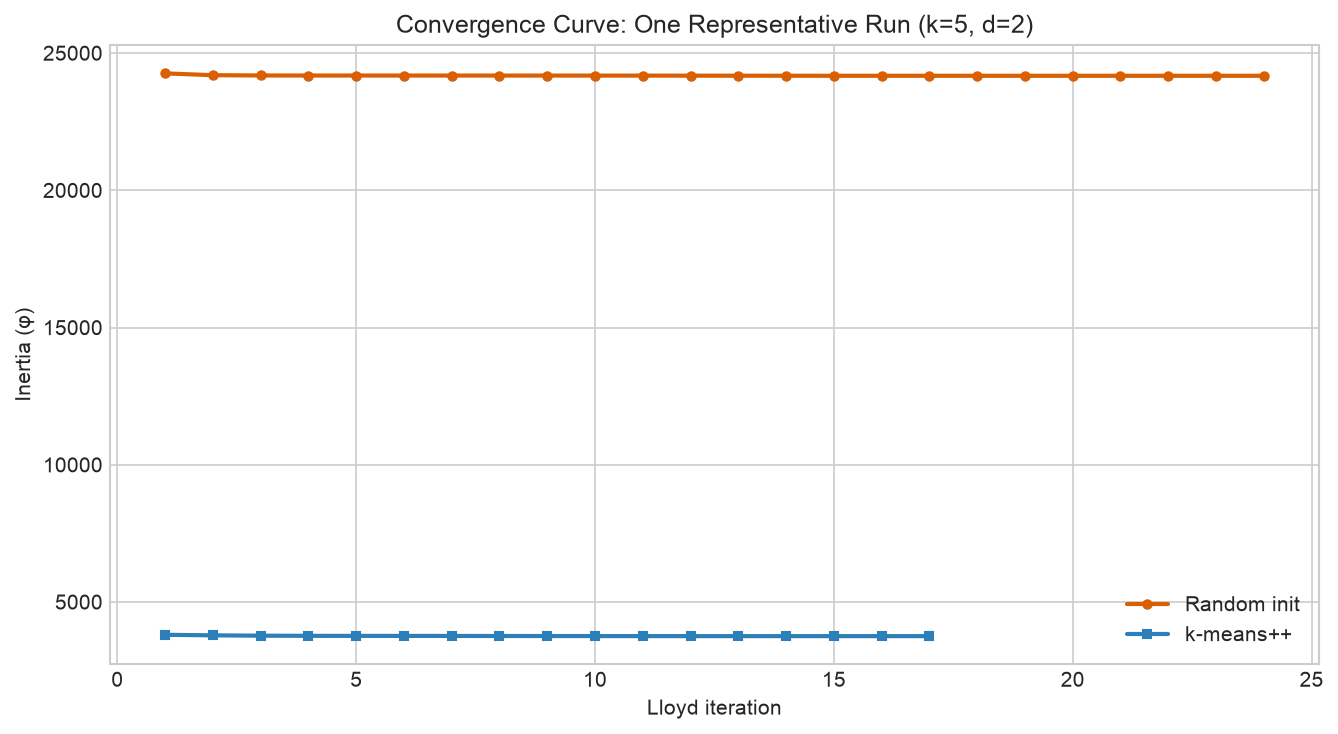
\includegraphics[width=\textwidth]{figures/synth_convergence.png}
    \caption{Convergence curve (one run each).}
  \end{subfigure}
  \hfill
  \begin{subfigure}[b]{0.48\textwidth}
    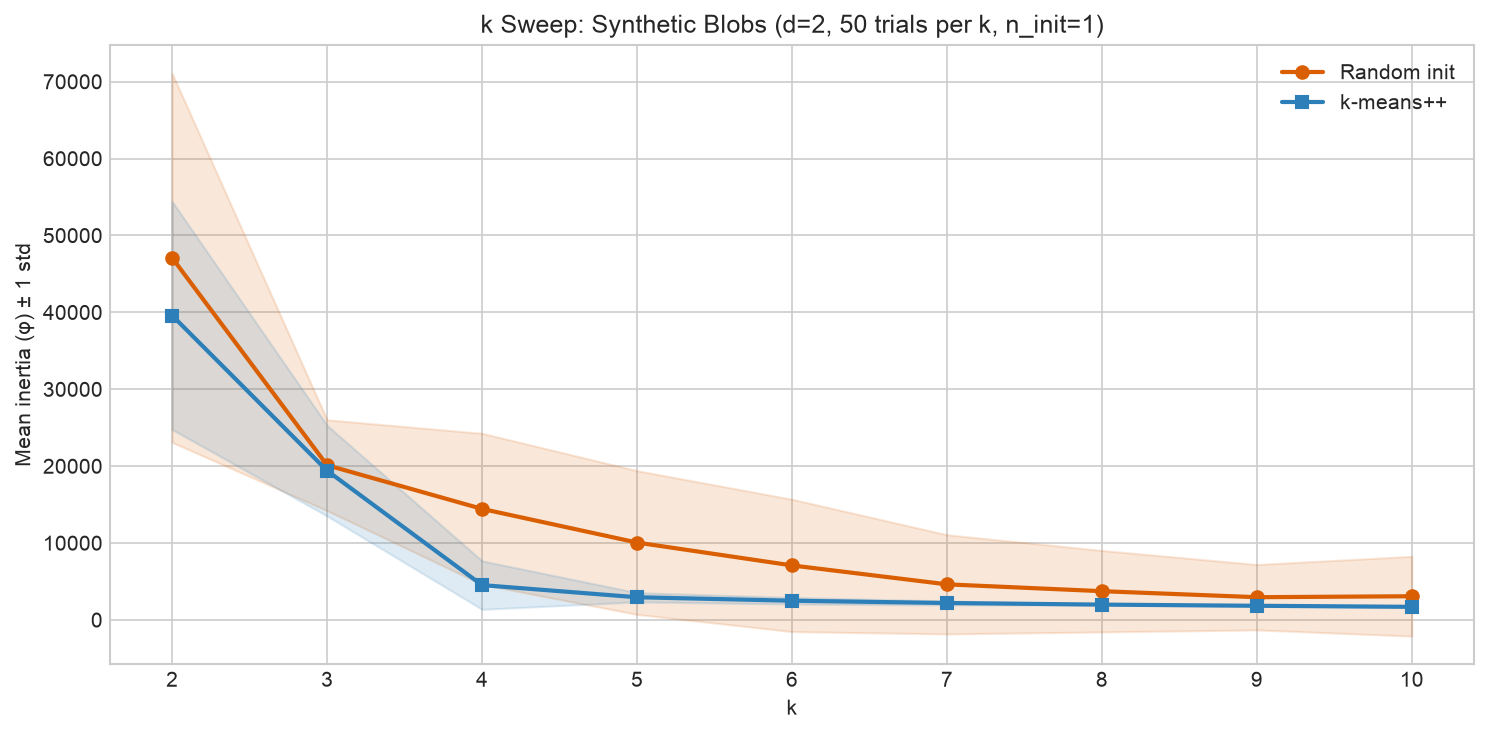
\includegraphics[width=\textwidth]{figures/synth_k_sweep.png}
    \caption{Mean inertia $\pm$ 1 std across $k$ (50 trials).}
  \end{subfigure}
  \caption{Convergence speed and k-sweep on synthetic blobs.}
  \label{fig:synth-convergence}
\end{figure}

k-means++ typically converged in fewer Lloyd iterations (\Cref{fig:synth-convergence},
left), on average 8.5 iterations versus 12.2 for random init over 100 trials,
matching the empirical findings in Table~1 of the paper.
The advantage in mean inertia is maintained across the full $k=2$--$10$
range (\Cref{fig:synth-convergence}, right), and the standard deviation
of k-means++ remains consistently lower, indicating more reliable solutions.

\paragraph{Extension: overlapping clusters ($\sigma=2.5$).}
When cluster boundaries overlap substantially the optimisation landscape
flattens and neither seeding strategy dominates.
\Cref{fig:synth-overlap} shows that at $\sigma=2.5$ the mean inertia ratio
narrows to $\approx 1.000$ (random mean $\phi=13{,}850.7$, k-means++ mean
$\phi=13{,}835.2$); the spread of both distributions is similar.
This confirms that D$^2$-sampling's advantage depends on there being clear
spatial gaps for the seeding to exploit.

\begin{figure}[h]
  \centering
  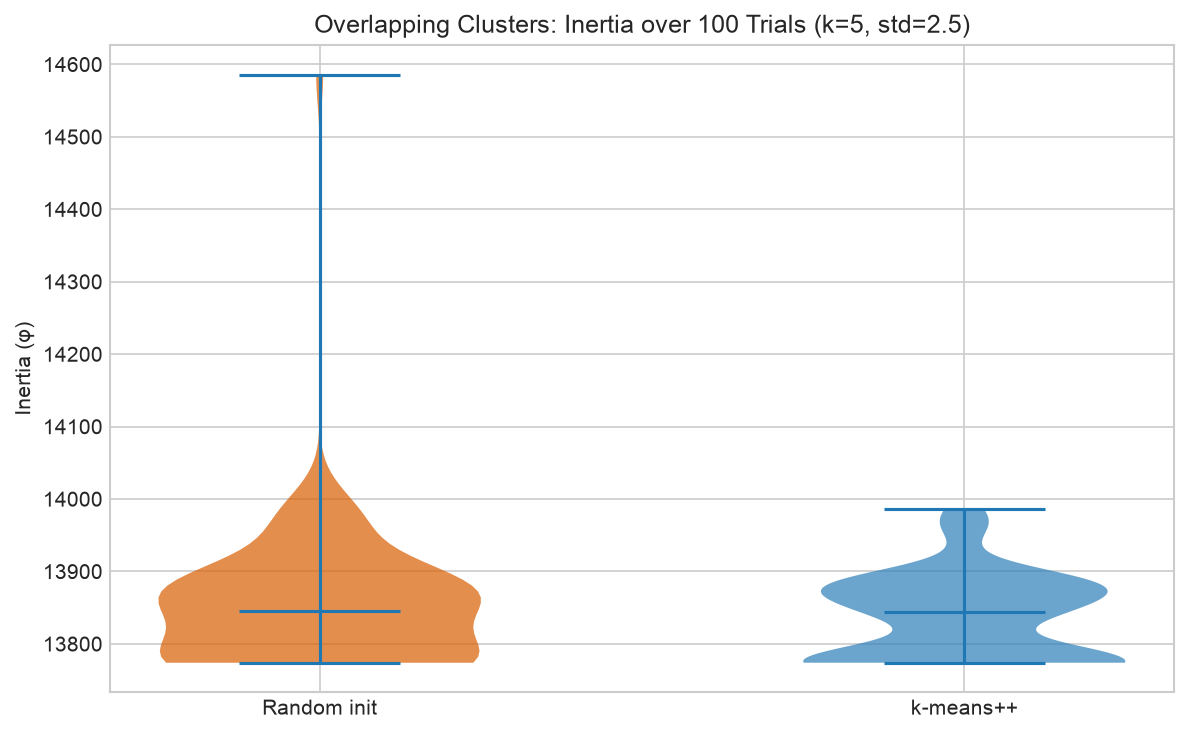
\includegraphics[width=0.6\textwidth]{figures/synth_overlapping.png}
  \caption{Inertia distribution on overlapping blobs ($\sigma=2.5$, $k=5$,
           100 trials). The gap between random init and k-means++ nearly
           vanishes when cluster boundaries are indistinct.}
  \label{fig:synth-overlap}
\end{figure}

% -----------------------------------------------------------------------
\section{Results: Credit Card Segmentation Dataset}
\label{sec:results-real}
% -----------------------------------------------------------------------

\begin{figure}[h]
  \centering
  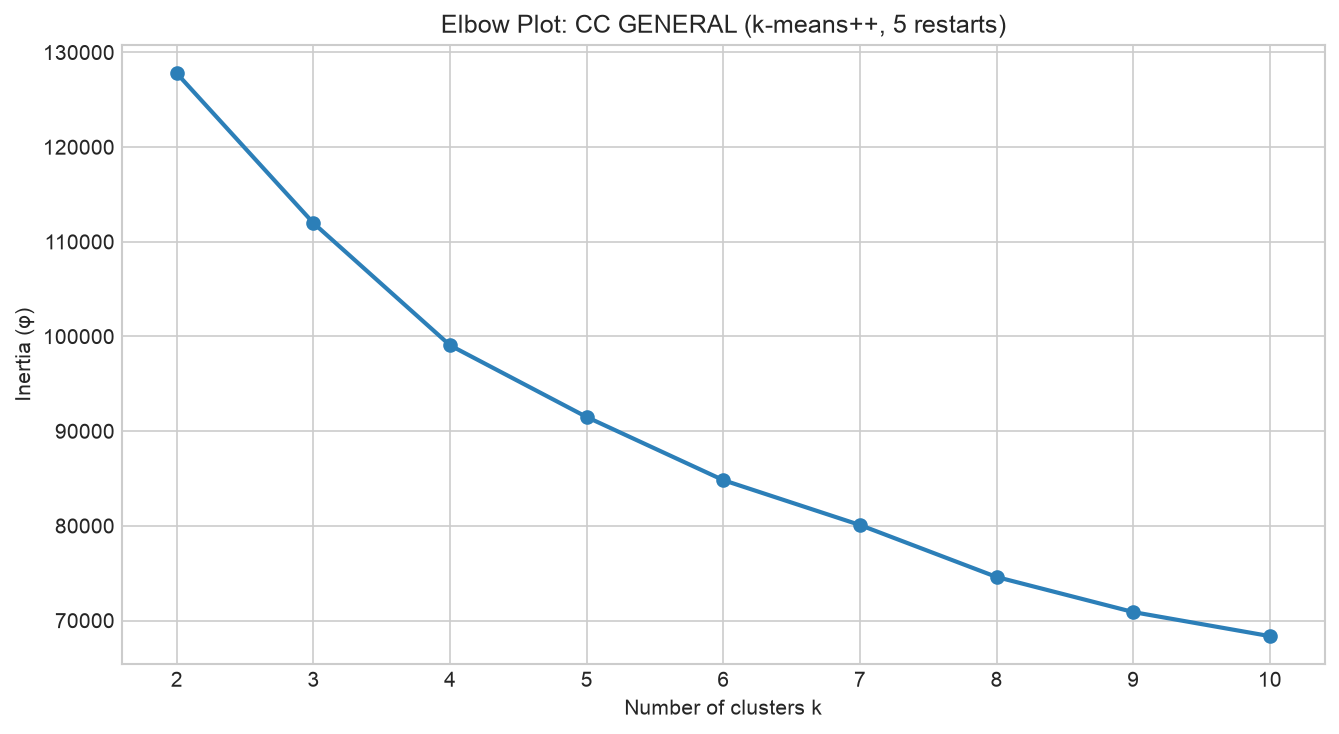
\includegraphics[width=0.55\textwidth]{figures/eda_elbow.png}
  \caption{Elbow plot on Credit Card Segmentation Dataset (k-means++, 5 restarts). The inflection
           at $k=3$ motivates using $k=3$ as the primary experimental focus.}
  \label{fig:eda-elbow}
\end{figure}

The elbow plot (\Cref{fig:eda-elbow}) shows a clear inflection at $k=3$,
which is therefore the primary focus of the initialisation comparison.

\begin{figure}[h]
  \centering
  \begin{subfigure}[b]{0.48\textwidth}
    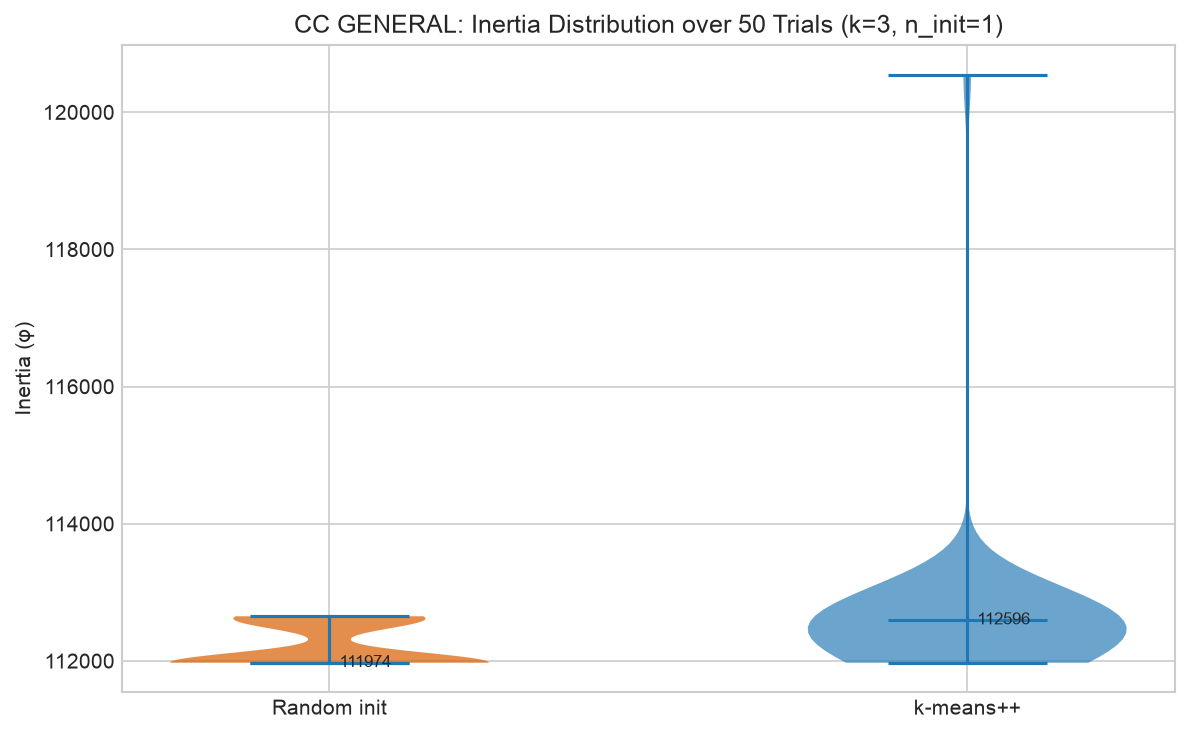
\includegraphics[width=\textwidth]{figures/real_inertia_violin.png}
    \caption{Inertia distribution over 50 trials ($k=3$, $n_\text{init}=1$).}
  \end{subfigure}
  \hfill
  \begin{subfigure}[b]{0.48\textwidth}
    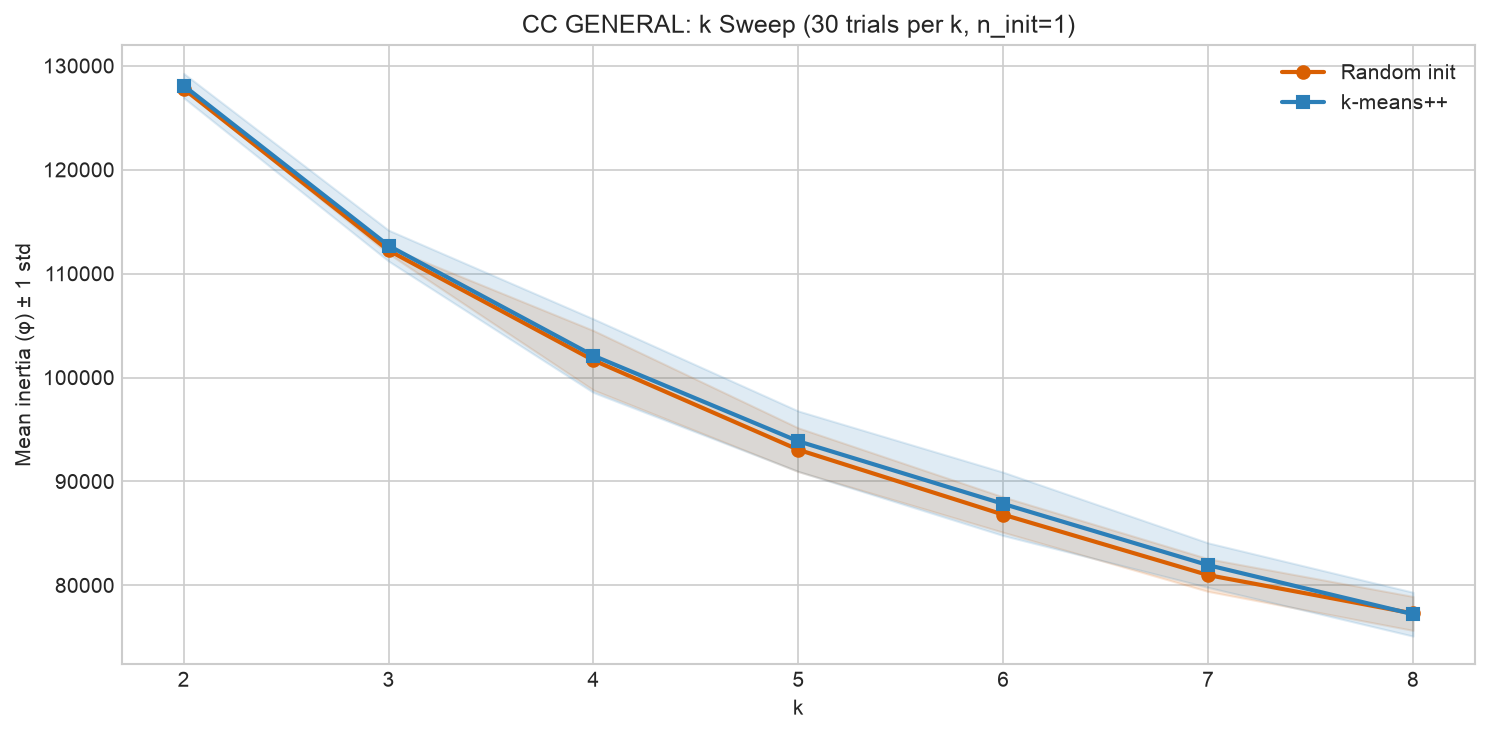
\includegraphics[width=\textwidth]{figures/real_k_sweep.png}
    \caption{k sweep ($k=2$--$8$, 30 trials per $k$).}
  \end{subfigure}
  \caption{Initialization comparison on Credit Card Segmentation Dataset.}
  \label{fig:real-violin}
\end{figure}

The Credit Card Segmentation Dataset results are more nuanced than the synthetic case.
Both methods find the same global optimum ($\phi = 111{,}973$), but at $k=3$
random initialisation achieves a \emph{lower} mean inertia ($112{,}218.9$
vs $112{,}577.9$) with substantially \emph{lower} variance (std $313.6$
vs $1{,}178.8$), a pattern that holds across the full $k=2$--$8$ sweep
(\Cref{fig:real-violin}).
This is not a failure of k-means++: when $k$ is small and the clusters are
well-separated, the optimisation landscape has few local minima and even
uniform random seeds rarely miss the global solution.
The k-means++ advantage in mean inertia reappears only at $k \geq 8$, where
the landscape becomes harder and D$^2$-sampling's spread helps more.
This qualifies the theoretical guarantee: Theorem~3.1 bounds the
\emph{expected} cost before Lloyd runs on a worst-case input; on an easy
instance with small $k$, the simpler baseline is equally reliable.

\begin{figure}[h]
  \centering
  \begin{subfigure}[b]{0.32\textwidth}
    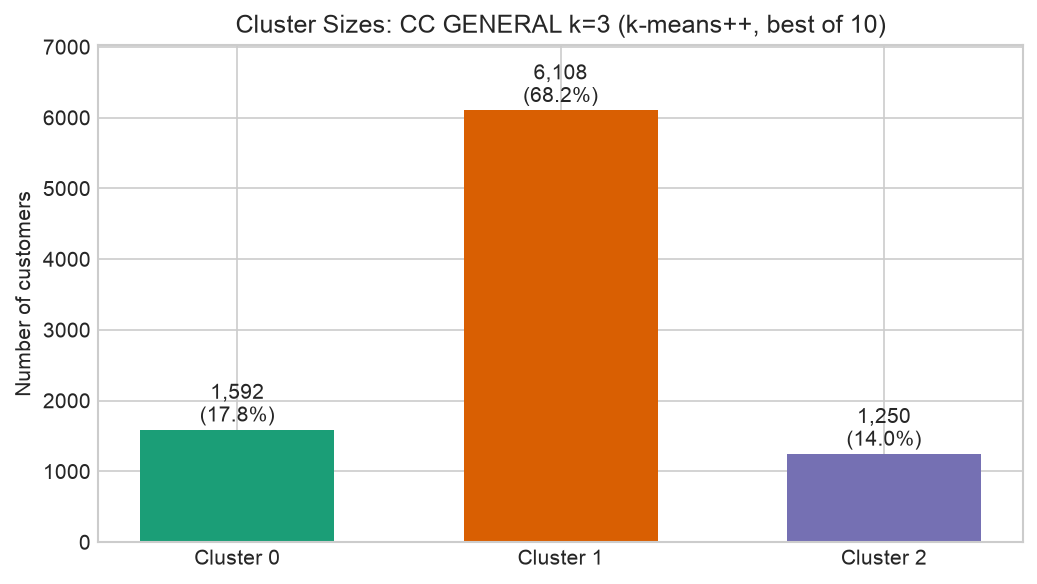
\includegraphics[width=\textwidth]{figures/real_cluster_sizes.png}
    \caption{Cluster sizes.}
  \end{subfigure}
  \hfill
  \begin{subfigure}[b]{0.64\textwidth}
    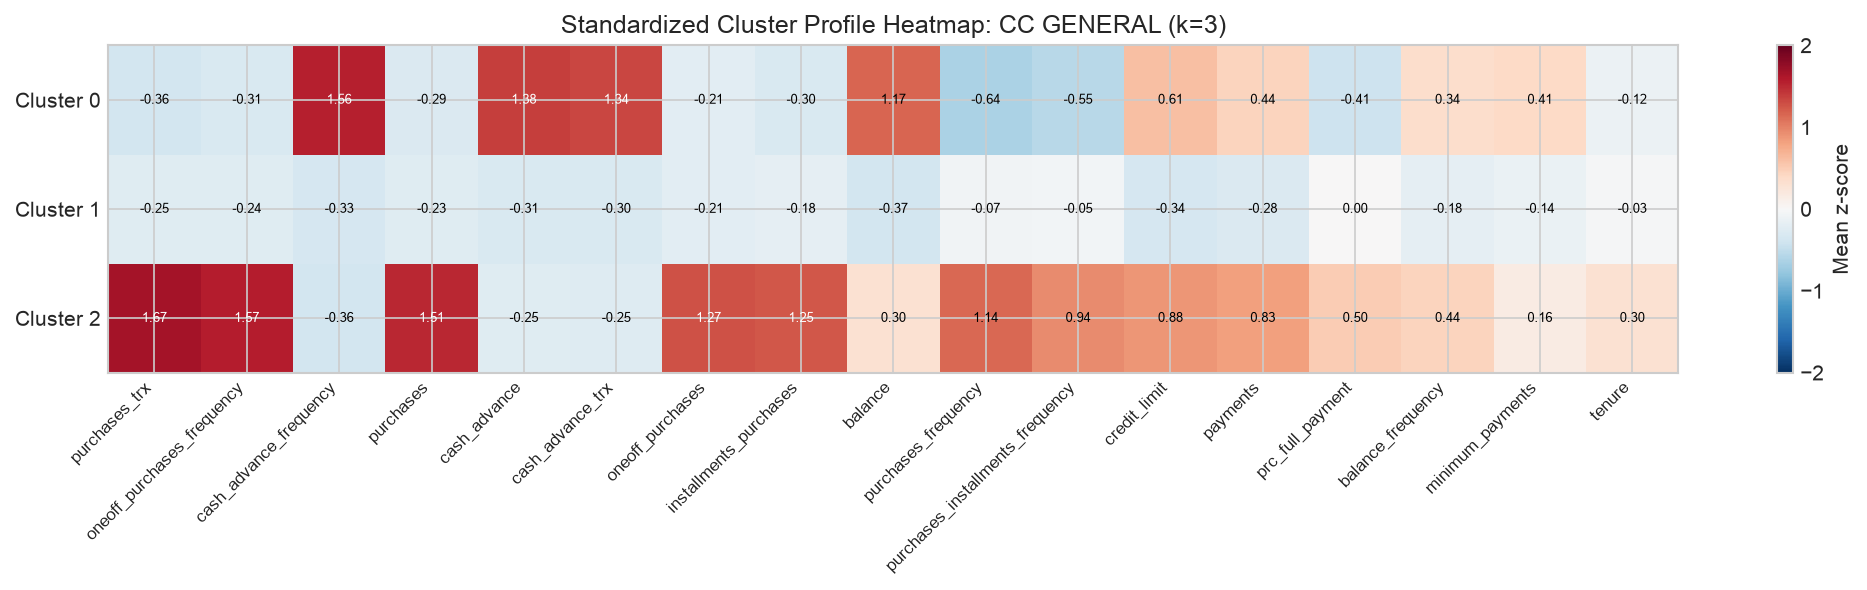
\includegraphics[width=\textwidth]{figures/real_heatmap.png}
    \caption{Standardised feature profile (mean z-score per cluster).}
  \end{subfigure}
  \caption{Best k-means++ solution ($k=3$, \texttt{n\_init=10}, silhouette $= 0.251$).}
  \label{fig:real-profile}
\end{figure}

The preferred solution ($k=3$, k-means++, 10 restarts) yields three
interpretable customer segments visible in \Cref{fig:real-profile}:

\begin{itemize}
  \item \textbf{Cluster 0} ($17.8\%$, $n=1{,}592$):
    \emph{Cash-advance-heavy customers}: mean balance $4{,}002$, mean cash
    advance $3{,}871$, low purchase activity (mean purchases $386$).
    High outstanding balance relative to payments.
  \item \textbf{Cluster 1} ($68.2\%$, $n=6{,}108$):
    \emph{Mainstream / moderate customers}: near-average on most features,
    mean balance $800$, mean purchases $502$, minimal cash-advance use.
    The largest segment by far.
  \item \textbf{Cluster 2} ($14.0\%$, $n=1{,}250$):
    \emph{Purchase-focused customers}: elevated purchase frequency and
    one-off purchase amounts, higher credit limits, low cash-advance usage.
\end{itemize}

The three segments are differentiated primarily along two behavioural axes
(purchase activity vs cash-advance reliance) that are visible in the
correlation blocks of the feature matrix, supporting the validity of $k=3$.

\begin{figure}[h]
  \centering
  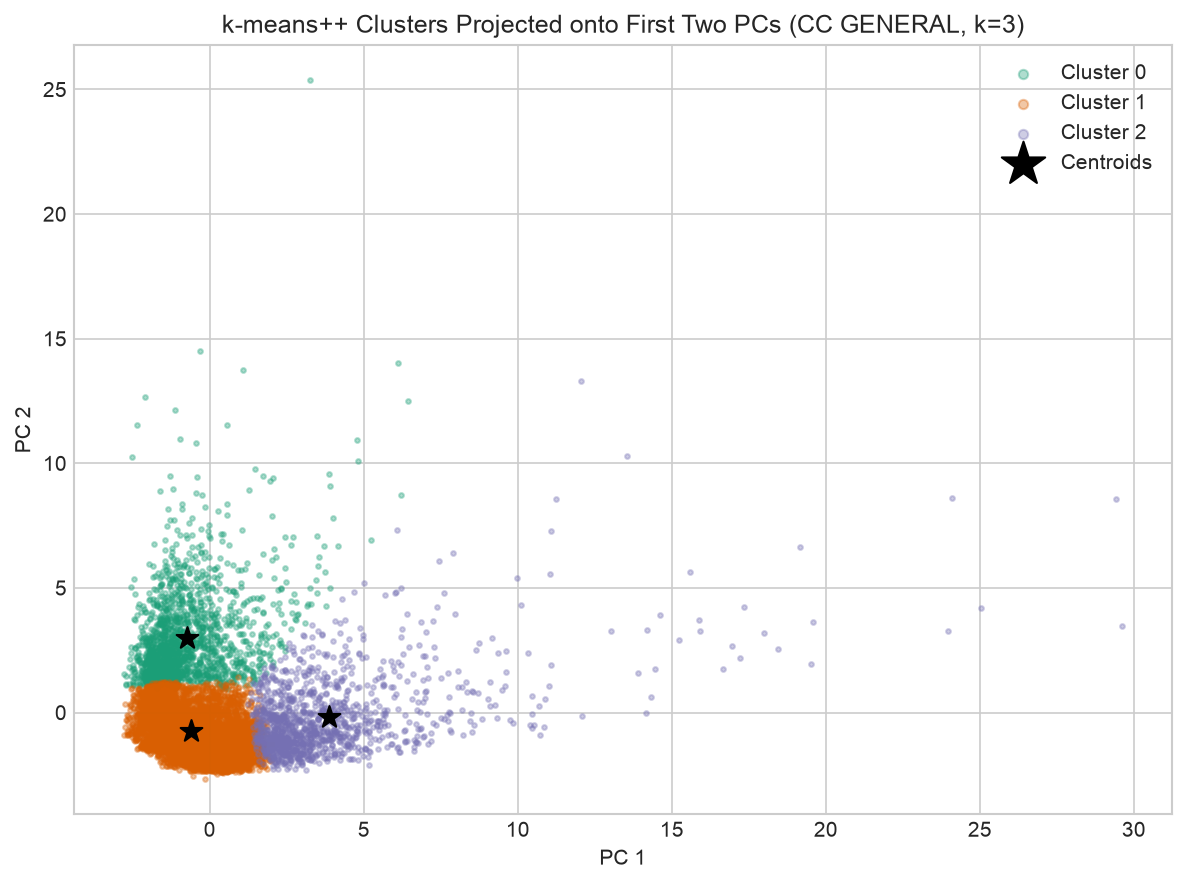
\includegraphics[width=0.65\textwidth]{figures/real_pca_scatter.png}
  \caption{k-means++ clusters projected onto the first two principal components
           (CC GENERAL, $k=3$). Stars mark centroids. The three segments
           separate clearly along PC~1, which correlates with cash-advance use.}
  \label{fig:real-pca}
\end{figure}

% -----------------------------------------------------------------------
\section{Results: MNIST Extension}
\label{sec:results-mnist}
% -----------------------------------------------------------------------

\begin{figure}[h]
  \centering
  \begin{subfigure}[b]{0.48\textwidth}
    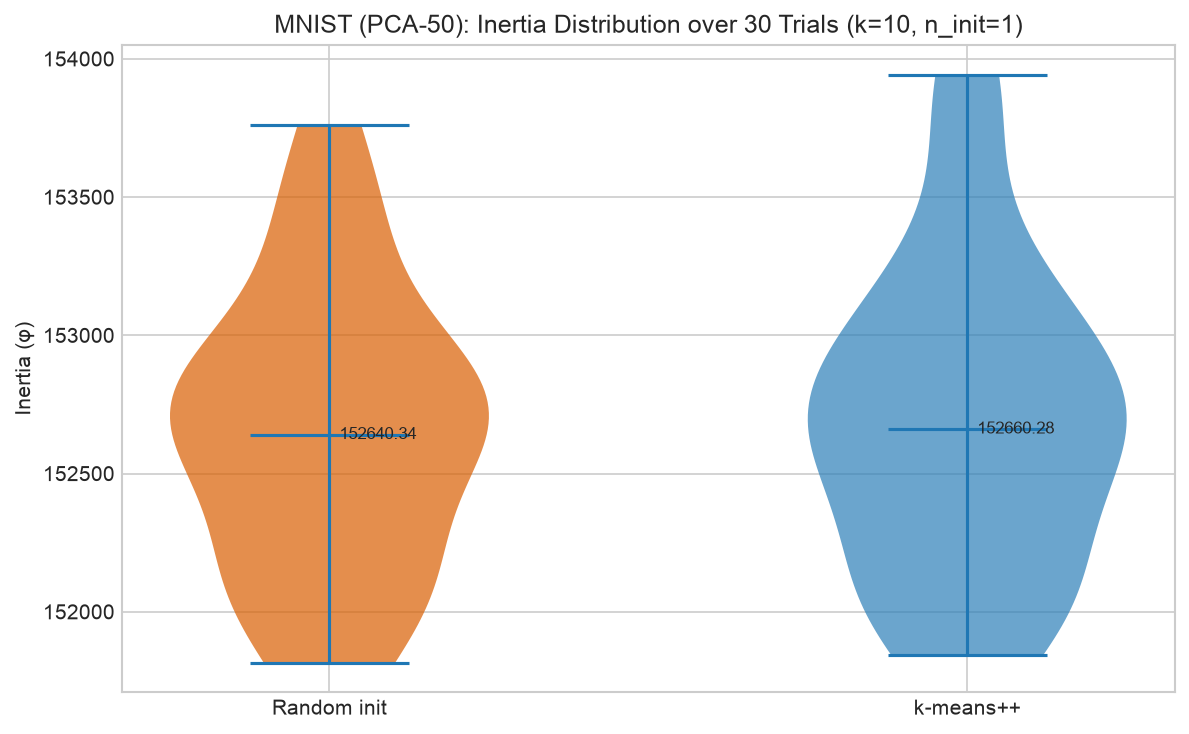
\includegraphics[width=\textwidth]{figures/mnist_inertia_violin.png}
    \caption{Inertia distribution ($k=10$, 30 trials, $n_\text{init}=1$).}
  \end{subfigure}
  \hfill
  \begin{subfigure}[b]{0.48\textwidth}
    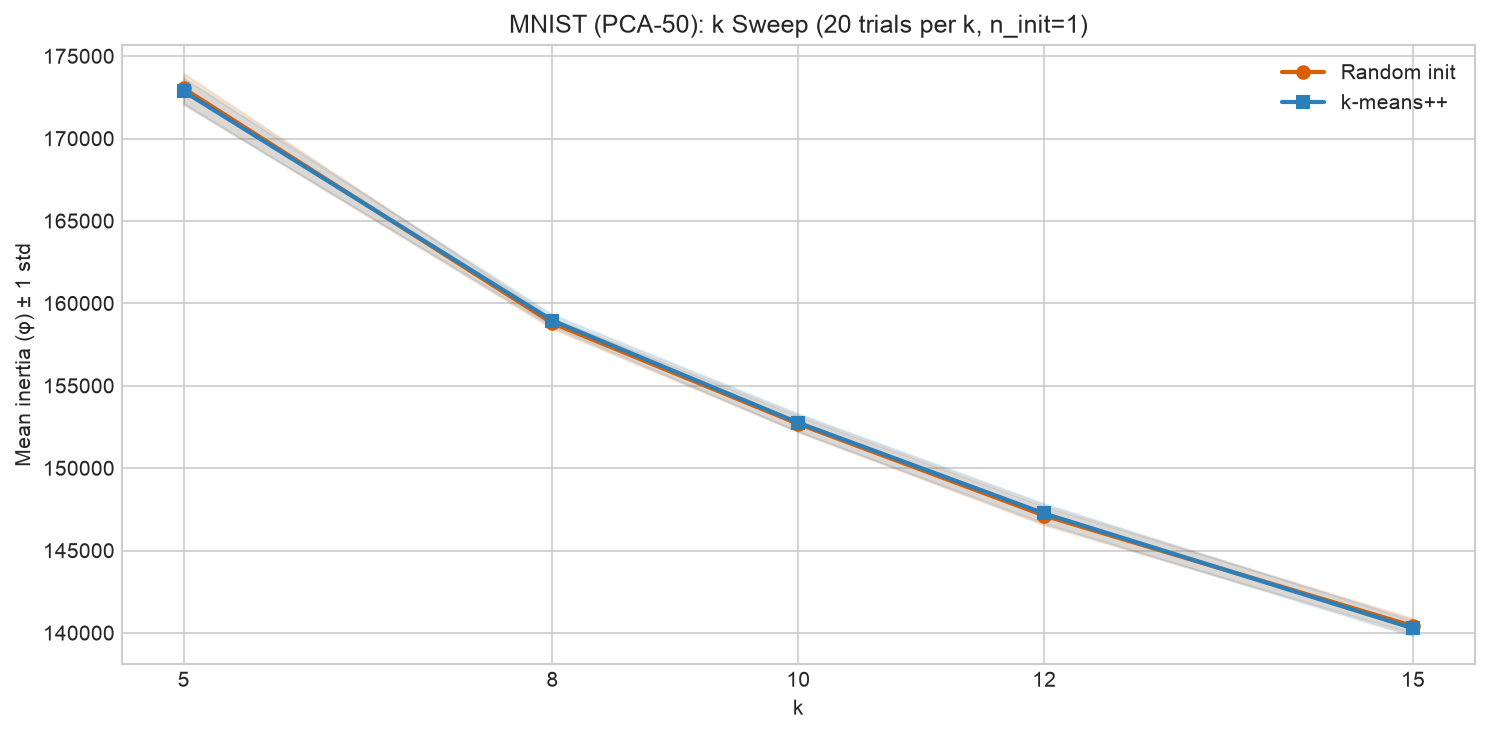
\includegraphics[width=\textwidth]{figures/mnist_k_sweep.png}
    \caption{k sweep ($k \in \{5,8,10,12,15\}$, 20 trials per $k$).}
  \end{subfigure}
  \caption{Initialization comparison on MNIST (PCA-50, $n=5{,}000$).}
  \label{fig:mnist-violin}
\end{figure}

In the 50-dimensional PCA space with $k=10$, the mean inertia ratio
(random / k-means++) is \textbf{1.000}: over 30 trials the two strategies
produce statistically indistinguishable inertia values
(random mean $152{,}652.6$ $\pm$ $507.4$; k-means++ $152{,}693.8$ $\pm$ $553.5$).
Both methods are solving an equally hard optimisation problem in this space,
and neither consistently finds a lower local minimum.

Cluster purity (sanity check only, using true digit labels) tells a different
story: with 10 restarts, k-means++ achieves \textbf{58.7\%} purity versus
random's \textbf{56.0\%}, meaning its assignments align better with the true
digit structure even when the inertia values are nearly equal.
This dissociation (similar inertia, better label alignment) suggests
that k-means++ finds a qualitatively different local minimum that better
respects the underlying manifold geometry of the digit images.
It is a concrete illustration that inertia alone does not fully characterise
clustering quality.

\begin{figure}[h]
  \centering
  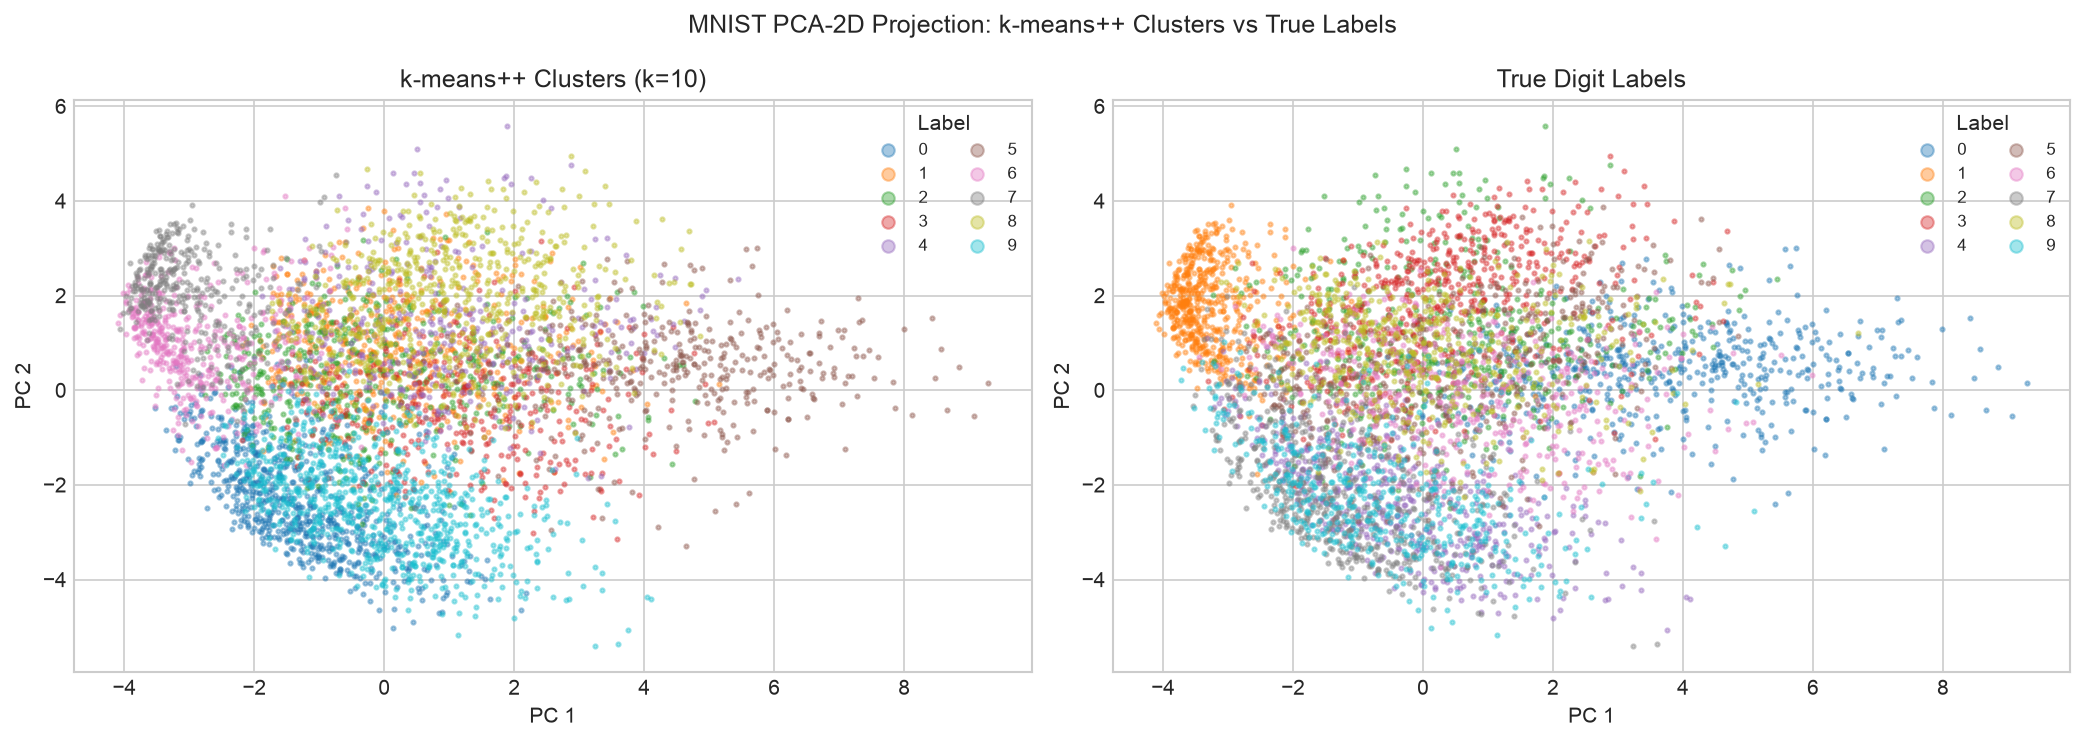
\includegraphics[width=0.9\textwidth]{figures/mnist_pca_scatter.png}
  \caption{MNIST (PCA-50) clusters in 2-D (left: k-means++ assignments,
           right: true digit labels). The broad agreement between the two
           panels confirms that k=10 clusters correspond loosely to the
           ten digit classes.}
  \label{fig:mnist-pca}
\end{figure}

% -----------------------------------------------------------------------
\section{Discussion}
% -----------------------------------------------------------------------

\paragraph{When does k-means++ help most?}
The experiments reveal that the advantage of k-means++ is context-dependent.
On synthetic blobs, the mean inertia ratio (random / k-means++) is
\textbf{3.09$\times$} at $d=2$ and grows to \textbf{4.54$\times$} at $d=20$,
confirming that D$^2$-sampling is particularly valuable in higher dimensions
where random seeding is more likely to cluster multiple initial centres near
the same region.
On the Credit Card Segmentation Dataset at small $k$, the advantage \emph{reverses}: random init is
more stable at $k=3$ because the landscape has few local minima and both
methods reliably find the global optimum.
In the MNIST high-dimensional setting at $k=10$, the inertia values are
indistinguishable but k-means++ produces better-aligned clusters, suggesting
the benefit manifests in solution quality rather than the inertia metric.

\paragraph{Does the O(log k) bound predict the observed ratio?}
Theorem~3.1 guarantees $\E[\phiC] \leq 8(\ln k + 2)\OPT$.
For $k=5$ this gives a worst-case factor of $8(\ln 5 + 2) \approx 28.9$.
The observed ratios of $3.09\times$ and $4.54\times$ are far below this bound,
confirming that the guarantee is a conservative worst-case estimate.
In practice the benefit is meaningful but modest, and disappears on easy
instances where the optimisation landscape is simple.

\paragraph{The Credit Card Segmentation Dataset finding as a case study.}
The real dataset reveals an important nuance not obvious from the theory:
when $k$ is small relative to the number of natural clusters and those clusters
are well-separated, random initialisation already finds the global minimum
reliably.
The k-means++ advantage is not universal: it is most pronounced when the
optimisation landscape is genuinely hard, i.e., when $k$ is large, the feature
space is high-dimensional, or the clusters overlap significantly.
Practitioners should consider the expected difficulty of their problem before
choosing between the two strategies, rather than defaulting to k-means++ in
all cases.

\paragraph{Limitations.}
Inertia is an internal measure that rewards tight clusters regardless of their
practical meaning, and there is no ground truth in the real-world setting.
The cluster profiles and purity results provide additional evidence, but
interpretation remains descriptive.
All distance-based methods are sensitive to feature scale, which is why
standardisation is a prerequisite; the results reported here may not transfer
to datasets where features require different normalisation choices.

% -----------------------------------------------------------------------
\section{Conclusion}
% -----------------------------------------------------------------------

We implemented k-means and k-means++ from scratch and evaluated them across
three settings: synthetic Gaussian blobs, the Credit Card Segmentation Dataset,
and MNIST.
The results support the theoretical guarantee of Theorem~3.1 but also reveal
its limits.
On synthetic data, k-means++ achieves inertia ratios of $3.09\times$ ($d=2$)
and $4.54\times$ ($d=20$) over random init, with faster convergence.
On the Credit Card Segmentation Dataset at $k=3$, both methods reach the same global optimum but random
init is more stable, an important qualifier: the D$^2$ guarantee bounds
the \emph{expected} cost on hard inputs, not the behaviour on easy ones.
On MNIST (PCA-50, $k=10$), the inertia advantage vanishes but k-means++
produces qualitatively better-aligned clusters (purity $58.7\%$ vs $56.0\%$),
a dissociation that inertia alone cannot detect.
Taken together, the results confirm that k-means++ is a robust improvement
over random seeding, but the magnitude and nature of the improvement depend
on the difficulty of the optimisation landscape, a practical nuance the
theoretical bound does not fully capture.

% -----------------------------------------------------------------------
\section*{Academic Integrity Declaration}
% -----------------------------------------------------------------------

\textit{I declare that this material, which I now submit for assessment,
is entirely my own work and has not been taken from the work of others, save
and to the extent that such work has been cited and acknowledged within the
text of my work. I understand that plagiarism, collusion, and copying are
grave and serious offences in the university and accept the penalties that
would be imposed should I engage in plagiarism, collusion or copying. This
assignment, or any part of it, has not been previously submitted by me or
any other person for assessment on this or any other course of study.}

% -----------------------------------------------------------------------
\bibliographystyle{plain}
\begin{thebibliography}{9}

\bibitem{arthur2007kmeans}
D.~Arthur and S.~Vassilvitskii.
\newblock k-means++: The advantages of careful seeding.
\newblock In \textit{Proceedings of the 18th Annual ACM-SIAM Symposium on
Discrete Algorithms (SODA)}, pages 1027--1035, 2007.

\bibitem{ccgeneral}
{Kaggle}.
\newblock Credit Card Dataset for Clustering.
\newblock \url{https://www.kaggle.com/datasets/arjunbhasin2013/ccdata}, 2018.

\bibitem{lecun1998mnist}
Y.~LeCun, L.~Bottou, Y.~Bengio, and P.~Haffner.
\newblock Gradient-based learning applied to document recognition.
\newblock \textit{Proceedings of the IEEE}, 86(11):2278--2324, 1998.

\end{thebibliography}

\end{document}
